\chapter{Implementación y Experimentos}\label{chapter:implementation}

% En este cap\'itulo de detalla la implementaci\'on de nuestra propuesta con la utilizaci\'on de AutoGOAL. Luego se realizan diferentes pruebas con datasets extaidos de la literatura contra varias m\'etricas y se analiza la efectividad de la propuesta.

% Aqui hablar de todo en general (para este viernes)
% Donde es que se engancha mi implementaci\'on 
% Pintar un diagrama de esto 
% Explicar todas las partes del diagrama

Se desarrola la propuesta sobre AutoGOAL un sistema de AutoML ideado en el grupo de Inteligencia Artificial de la Universidad de la Habana.
Se aplica el sistema sobre tres corupus distintos junto con dos pares de m\'etricas para comprobar el rendimiento.

\section{Implementaci\'on}


AutoGOAL es un sistema de AutoML gen\'etico que utiliza una Gram\'atica Probabil\'istica Libre del Contexto  para modelar su espacio de decisi\'on. Se representa utilizando un grafo aciclico dirigido (DAG) donde cada nodo de este representa una posible cadena de la gram\'atica y sus aristas apuntan a todas las posibles cadenas que se pueden generar a partir de estas sustituyendo alg\'un No Terminal por una producci\'on de la Gram\'atica. Cuando una cadena se encuentra completamente expandida, i.e. compuesta por solo simbolos terminales, se tiene una soluci\'on v\'alida del sistema. 

Inicialmente cada arista de este DAG se inicializa con una probabilidad igual a todas sus aristas hermanas (i.e. todas las aristas que salen de su mismo nodo) tal que la suma de sus probabilidades sea 1. Un camino se escoge utilizando una variable uniforme tal que su valor determina la arista a seleccionar. Cuando se tiene un individuo apto la manera de AutoGOAL de conservar sus ``genes'' es aplicando PGE sobre las aristas que conforman el camino que llevaron a esa soluci\'on. M\'as especificamente, la implementaci\'on de AutoGOAL de PGE dado $n$ individuos, son evaluados respecto a una funci\'on de evaluaci\'on $f$ y se crea una listas de las $k$ mejores soluciones (encabezada por la m\'as apta) y las aristas de las probabilidades se actualizan de acuerdo a estas soluciones. 

Se a\~nade a AutoGOAL la clase NSPGE, un m\'etodo de b\'usqueda inspirado en NSGA-II (\cite{deb2002fast}) que utiliza PGE como base. El objetivo de NSPGE es extender la funcionalidad de PGE para que sea capaz de seleccionar los $k$ mejores individuos de acuerdo a $m$ m\'etricas, con $m \ge 2$. La l\'ogica de la PGE encargada de ordenar los inidividuos m\'as aptos se encuentra en el m\'etodo \textit{\_inidices\_of\_the\_fittest\_} la cual NPSGE sobreescribe.

\subsection{Nueva ordenaci\'on}

En NSPGE, dentro de \textit{\_inidices\_of\_the\_fittest\_} se aplica la ordenaci\'on definida por \cite{deb2002fast}. Dado $n$ soluciones se  agrupan seg\'un su \'indice de dominaci\'on (i.e. Non Dominated Sorting), donde cada agrupamiento se le llama frente de rango $i$, donde $i$ representa la cantidad de soluciones que dominan a cada una de estas. Una vez establecidos estos frentes se extraen las primeras $k$ soluciones, en caso de que no se pueda seleccionar un frente completo, se aplica Crowding Distance para seleccionar la muestra m\'as representativa de este.

Es importante entender para la correctitud del aloritmo  que las soluciones que conforman un frente de rango $i$ no se \textit{Pareto dominan} ($\prec$) entre si.
%Es f\'acilmente demostrable que la \texit{Pareto dominacion (i.e. $\prec$)} cumple con la propiedad de transitividad (i.e. si $x \prec y$, $y \prec z$, entonces $x \prec z$) 
Dado un frente de rango $i$ $F_i$, tal que existen soluciones $x, y \in F_i$ se asume que $x \prec y$. Como el \'inidice de dominaci\'on de $x$ es $i$ y $x \prec y$ y ($\prec$) es una operador transitivo entonces todos los que dominan a $x$ dominan a $y$, adem\'as del propio $x$, por tanto el inidice de dominaci\'on de $y$ ser\'ia $i+1$ lo que es una contradicci\'on porque $y \in F_i$. 

\begin{lstlisting}[language=Python]
def _indices_of_fittest(self, fns: List[List[float]]):
  # Se ordenan todas las soluciones segun su orden
  # de dominacion
  fronts = self.non_dominated_sort(fns)
  indices = []
  k = int(self._selection * len(fns))

  for front in fronts:
    if len(indices) + len(front) <= k:
      indices.extend(front)
    else:
      # Cuando solo se utiliza una porcion del frente
      # se aplica crowding distance
      indices.extend(
          sorted(
              front,
              key=lambda i: -self.crowding_distance(fns, front, i)
          )[: k - len(indices)]
      )
      break
  return indices
\end{lstlisting}

\subsubsection{Non Dominated Sort}
La ordenaci\'on se conforma por dos pasos l\'ogicos fundamentales:
\begin{enumerate}
    \item Se verifica todo par de soluciones $x, y$ encontradas y se aplica $x \prec y$ con el objetivo de calcular el \'inidice de dominaci\'on de cada soluci\'on. Adem\'as se construye un DAG conformado por las soluciones donde existe una arista entre las soluciones $x$ y $y$ si $x \prec y$. La ra\'iz de dicho DAG est\'a conformado por las soluciones que nadie domina.
    \item Se recorre DAG utilizando una versi\'on de BFS ($Breadth First Search$) donde los soluciones visitadas se les reduce el \'indice de domianci\'on en uno. Si llega a 0 se a\~nade al frente de Pareto que se est\'a formando.
\end{enumerate}

\begin{lstlisting}[language=Python]
def non_dominated_sort(self, scores: List[List[float]]):
  # fronts almacena los frentes 
  #(i.e. fronts[i] es el frente de rango i)
  fronts: List[List[int]] = [[]]

  # domination_rank en i indica la cantidad de soluciones
  # que dominan a la solucion i
  domination_rank = [0] * len(scores)

  # dominated_scores en i alamacena las soluciones dominadas
  # por la solucion i
  dominated_scores = [list() for _ in scores]

  # revisa todo par de soluciones y se establece
  # quien dominan a quien
  for i, score_i in enumerate(scores):
    for j, score_j in enumerate(scores):
      if self._improves(score_i, score_j):
          dominated_scores[i].append(j)
      elif self._improves(score_j, score_i):
          domination_rank[i] += 1
    if domination_rank[i] == 0:
       fronts[0].append(i)

  # de acuerdo a la informacion sobre quienes
  # se dominan, forma todos los frentes
  front_rank = 0
  while len(fronts[front_rank]) > 0:
    next_front = []
    for i in fronts[front_rank]:
      for dominated in dominated_scores[i]:
        domination_rank[dominated] -= 1
        if domination_rank[dominated] == 0:
          next_front.append(dominated)
    front_rank += 1
    fronts.append(next_front)

  return fronts[:-1]
\end{lstlisting}

\subsubsection{Crowding Distance}
Se sigue la idea del algoritmo propuesto en (\ref{proposal:alg:cd}). Dado $m$ m\'etricas a evaluar se realizan $m$ iteraciones, donde en cada una se ordena alg\'un frente de rango $k$ de acuerdo a la metrica $m_i$. A la soluciones que con respecto a la m\'etrica $m_i$ tienen el m\'inimo y mayor valor se les asigna distancia infinita y luego se c\'alculan los valores intermedios. En \cite{deb2002fast} requiren que los valores de las m\'etricas esten normalizados, en nuestra implementaci\'on utilizamos \textit{feature scaling} para normalizar los valores entre 0 y 1.

\begin{lstlisting}[language=Python]
def crowding_distance(
    self, scores: List[List[float]], front: List[int], index: int
) -> float:
  # Crowding distance usa los vectores normalizados.
  # Se aplica feature scaling para llevar los vectores a [0, 1]
  scaled_scores = feature_scaling(scores)

  crowding_distances: List[float] = [0 for _ in scores]
  for m in range(len(self._maximize)):
    # Se ordena de acuerdo a la metrica m
    front = sorted(front, key=lambda x: scores[x][m])

    # Se establecen los extremos como infinitos
    crowding_distances[front[0]] = math.inf
    crowding_distances[front[-1]] = math.inf

    # Valores de todas las soluciones con respecto a m 
    m_values = [scaled_scores[i][m] for i in front]
    scale: float = max(m_values) - min(m_values)
    if scale == 0:
      scale = 1
    for i in range(1, len(front) - 1):
      crowding_distances[i] += (
        scaled_scores[front[i + 1]][m] - scaled_scores[front[i - 1]][m]
      ) / scale

  return crowding_distances[index]
\end{lstlisting}

\section{Marco Experimental}

En este secci\'on se analiza el desemepe\~no de la propuesta utilizando AutoGOAL.

El objetivo es ejecutar datasets distintos con diferentes m\'etricas de evaluaci\'on.

\subsection{M\'etricas Utilizadas}

Para cada conjutno de datos se utilizan los siguentes pares de m\'etricas:

\paragraph{Precision contra Recobrado}: Precisi\'on es cuando . Recobrado es cuando . Para los tests donde se utiliza de una manera. Y para otros de otra

\paragraph{F-Score contra Tiempo de Entrenamiento}: Se compara F-Score lo mismo que Recobrado y Precision. Para algunos tests de alguna forma, para otros de otra. Tiempo de Entrenemaiento es un estimado de cuanto timepo toma entrenar y validar el modelo.

\subsection{Corpus de Evaluaci\'on}

Se utilizan dos corpus de datos para comprobar el comportamiento del sistema cuando optmiza para varias m\'etricas simult\'aneamente.

\subsubsection{CARS}
Cars representa una conjunto de carros y con ciertas caracter\'isticas cat\'alogadas cualitativamente (ver \ref{implementation:table:cars:attributes}). Cada carro se clasifica de acuerdo a sus atributos  en inaceptable, aceptable, bueno o muy bueno (\ref{implementation:table:cars:classes}). El dataset no tiene valores desconocidos.

\begin{table}[ht]
    \centering
    \parbox{.45\linewidth}{
    \begin{tabular} { |l|c| }
        \hline
        Atributos & Valores \\
        \hline
        \hline
        buying & v-high, hihg, med, low \\
        \hline
        maintance &  v-high, hihg, med, low\\
        \hline
        doors & 2, 3, 4, 5-more\\
        \hline
        persons & 2, 4, more\\
        \hline
        lug\_boot & small, med, big\\
        \hline
        safety & low, med, high\\
        \hline
    \end{tabular}
    \caption{Tipos de Atributos en Cars}
    \label{implementation:table:cars:attributes}
    }
    \qquad
    \parbox[t]{.45\linewidth}{
    \begin{tabular} {|l|c|c|}
        \hline
        Clases & N & \% \\
        \hline
        \hline
        unacc & 1210 & 70.023\%\\
        \hline
        acc & 384 & 22.222\%\\
        \hline
        good & 69 & 3.993\%\\
        \hline
        v-good & 65 & 3.762\%\\
        \hline
    \end{tabular}
    \caption{Distribuci\'on de clases en Cars}
    \label{implementation:table:cars:classes}
    }
\end{table}

\subsubsection{HAHA}
Humor Analysis based on Human Annotation (HAHA), un conjunto de datos que contiene \textit{tweets} en espa\~nol y se clasifican en si son humor\'isticos o no. Contiene un total de 30000 tweets donde se utilizan 24000 para entrenaiento y 6000 para evaluaci\'on.

\begin{table}[ht]
    \centering
    \begin{tabular} {|l||c|c|c|}
        \hline
        & Entrenamiento & Evaluaci\'on & Total \\
        \hline
        \hline
        Tweets & 24000 & 6000 & $30000$\\
        \hline
        Graciosos & 9253 & 2342 & 11595\\
        \hline
        No graciosos & 14 757 & 3 658 & 18 405\\
        \hline
        Puntuaci\'on Promedio & 1305 & 275 & 1580\\
        \hline
    \end{tabular}
    \caption{Distribuci\'on de clases en HAHA}
    \label{implementation:table:haha}
\end{table}

\subsubsection{MEDDOCAN}

Una colecci\'on de 1000 casos cl\'inicos y sus anotaciones PHI; cada uno conformado con aproximadamente de 33 oraciones o 495 palabras. Cada caso cl\'inico est\'a codificado en texto plano en UTF8 y las anotaciones est\'an en formato BRAT.


\subsection{Configuraci\'on Experimental}

\paragraph{Hardware} Los experimentos fueron ejecutados en un equipo con las siguientes propiedades: CPU AMD R5 3550h y 32 GB de RAM.

\section{Resultados y An\'alisis}

A continuaci\'on se muestran los resultados y anal\'isi de aplicar autogoal con optimizaci\'on multiobjetivo a los distintos corpus. En las gr\'aficas solo se tiene en cuenta la puntuaci\'on respecto a los datos entrenamiento y no a los datos de prueba. Los puntos con tonalidades de grises marcan las mejores soluciones encontradas en cada generaci\'on que realiz\'o el sistema. La tonalidad de los puntos oscurecen a medida que han sido m\'as generaciones. Las puntos m\'as oscuros corresponden a iteraciones posteriores. Finalmente los puntos marcados con cruces rojas representan las mejores soluciones encontradas por el algoritmo y conforman una aproximaci\'on del frente de Pareto.

\subsection{Cars}

Se utilzo una poblacion total de 40 individuos, 1 hora de tiempo m\'aximo y 10 segundos de tiempo l\'imite por \textit{pipeline}. Se utilizaron las la implementaciones de \textit{f-score}, \textit{precision} y \textit{recall} de scikit-learn con el promedio \textit{weighted} utilizado para problemas de clasificaci\'on multiclase que pueden tener un desbalance en las clases existentes.

\subsubsection{F-Score contra Tiempo de Entrenamiento}

En la figura \ref{impl:fig:cars:fscore_vs_time} se observa que se obtiene una porci\'on aproximaci\'on del frente de Pareto bien distribuida. Se nota lo que se conoce en la literatura como un frente c\'oncavo. Ademas se puede ver como se tienen solucioens para escoger/ Desde cercanas a los milisegundos con una puntuaci\'on de 0.9, o que se peguen a los 0.2 milisegundos con una puntacion f casi perfecta. En este caso la diferencia de tiempe es negligible. No obstante al optimziar sim\'ulataneamete para el tiempo se evita que el algoritmo escoja caminos m\'as caros en tiempo como se ve en la columna de puntos a la derecha. Varios algoritmos con muy buena puntuaci\'on pero que se demoran 5 veces m\'as que el m\'as r\'apido.

% (hablar sobre los mejores algorimtos)?

\begin{figure}[ht]
    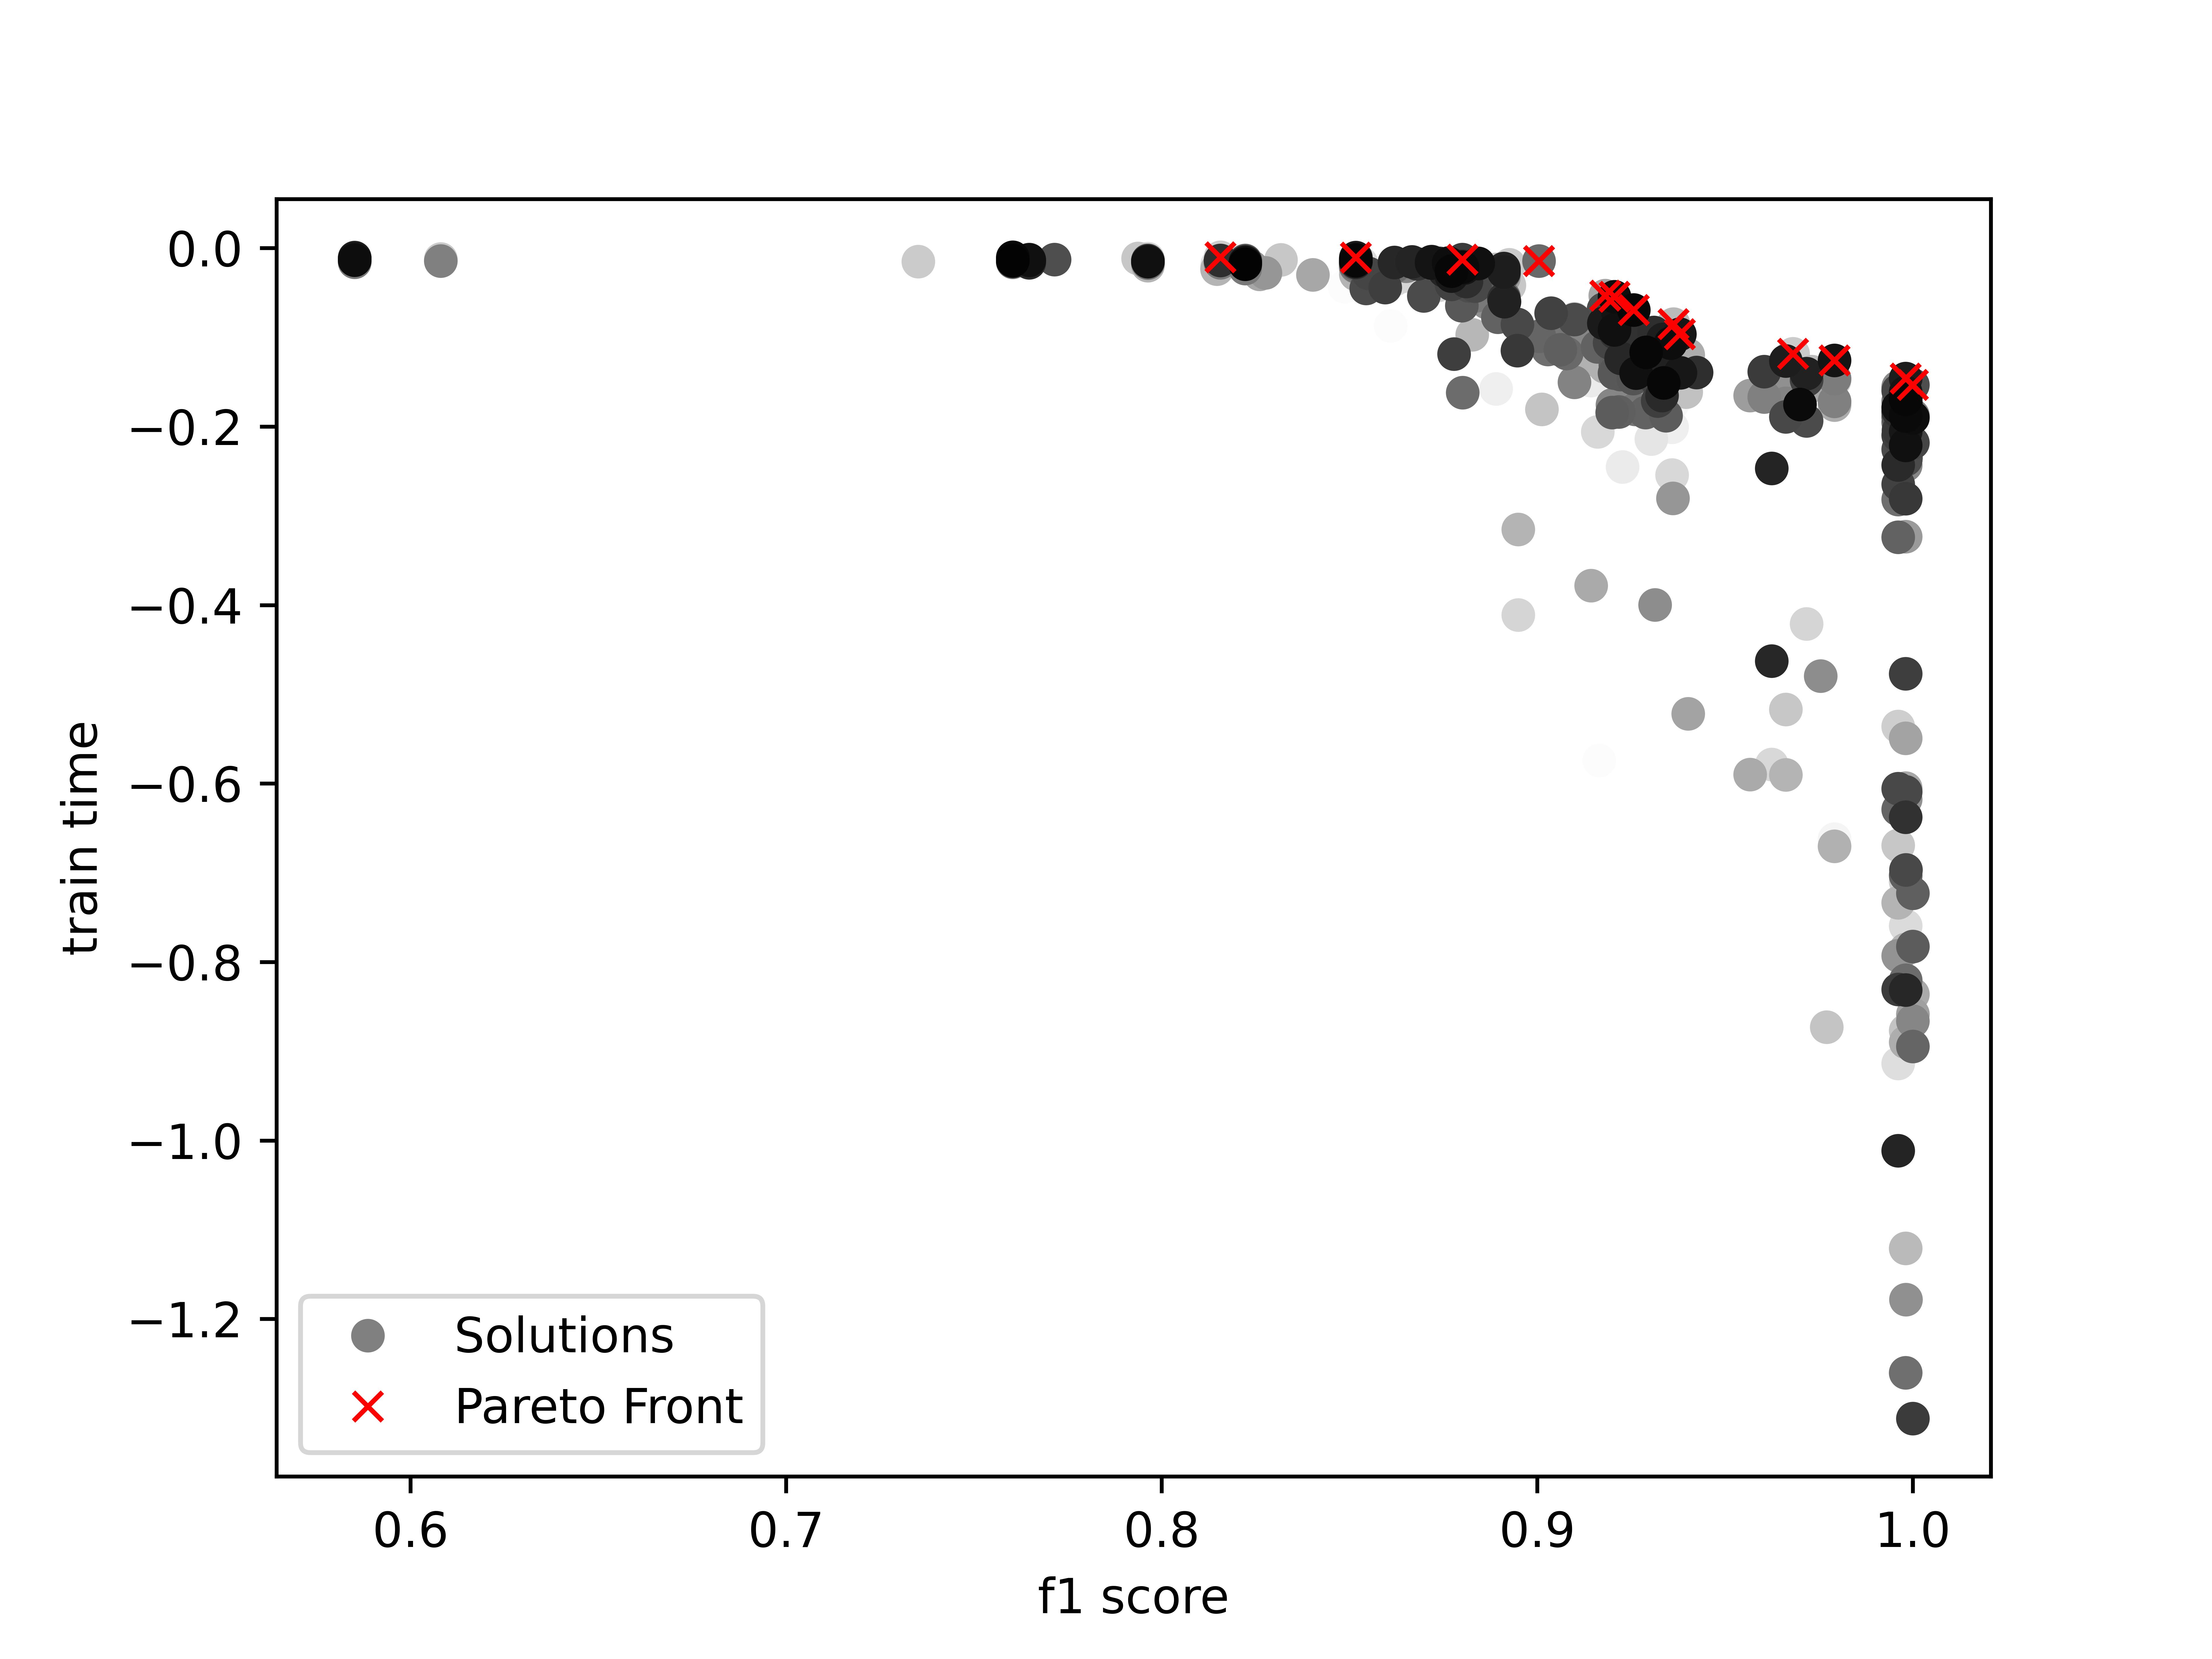
\includegraphics[width=\linewidth]{Pictures/cars_fscore_vs_time.jpg}
    \caption{Cars: f-score contra tiempo de entrenamiento}
    \label{impl:fig:cars:fscore_vs_time}
\end{figure}


\subsubsection{Precisi\'on contra Recobrado}

Este es un caso donde las m\'etricas a evaluar no entran en conflicto y no hay que hacer trade offs entre estas. Como se observa en \ref{impl:fig:cars:precision_vs_recall} el frente de Pareto esta consituido por un s\'olo punto tal que precision y recobrado son ambos el maximo. Se observa como en el transcrso de las generaciones las soluciones se acercan cada vez m\'as al frente de Pareto.

En este caso especif\'ico AutoGOAL encontr\'o 30 soluciones distintas con respecto a algoritmos e hyperpar\'ametros que logran este rendimiento. Puede haber ocasiones donde esto sea interesante para el usuario desde un punto de vista investigativo, ver en que difieren.


\begin{figure}[ht]
    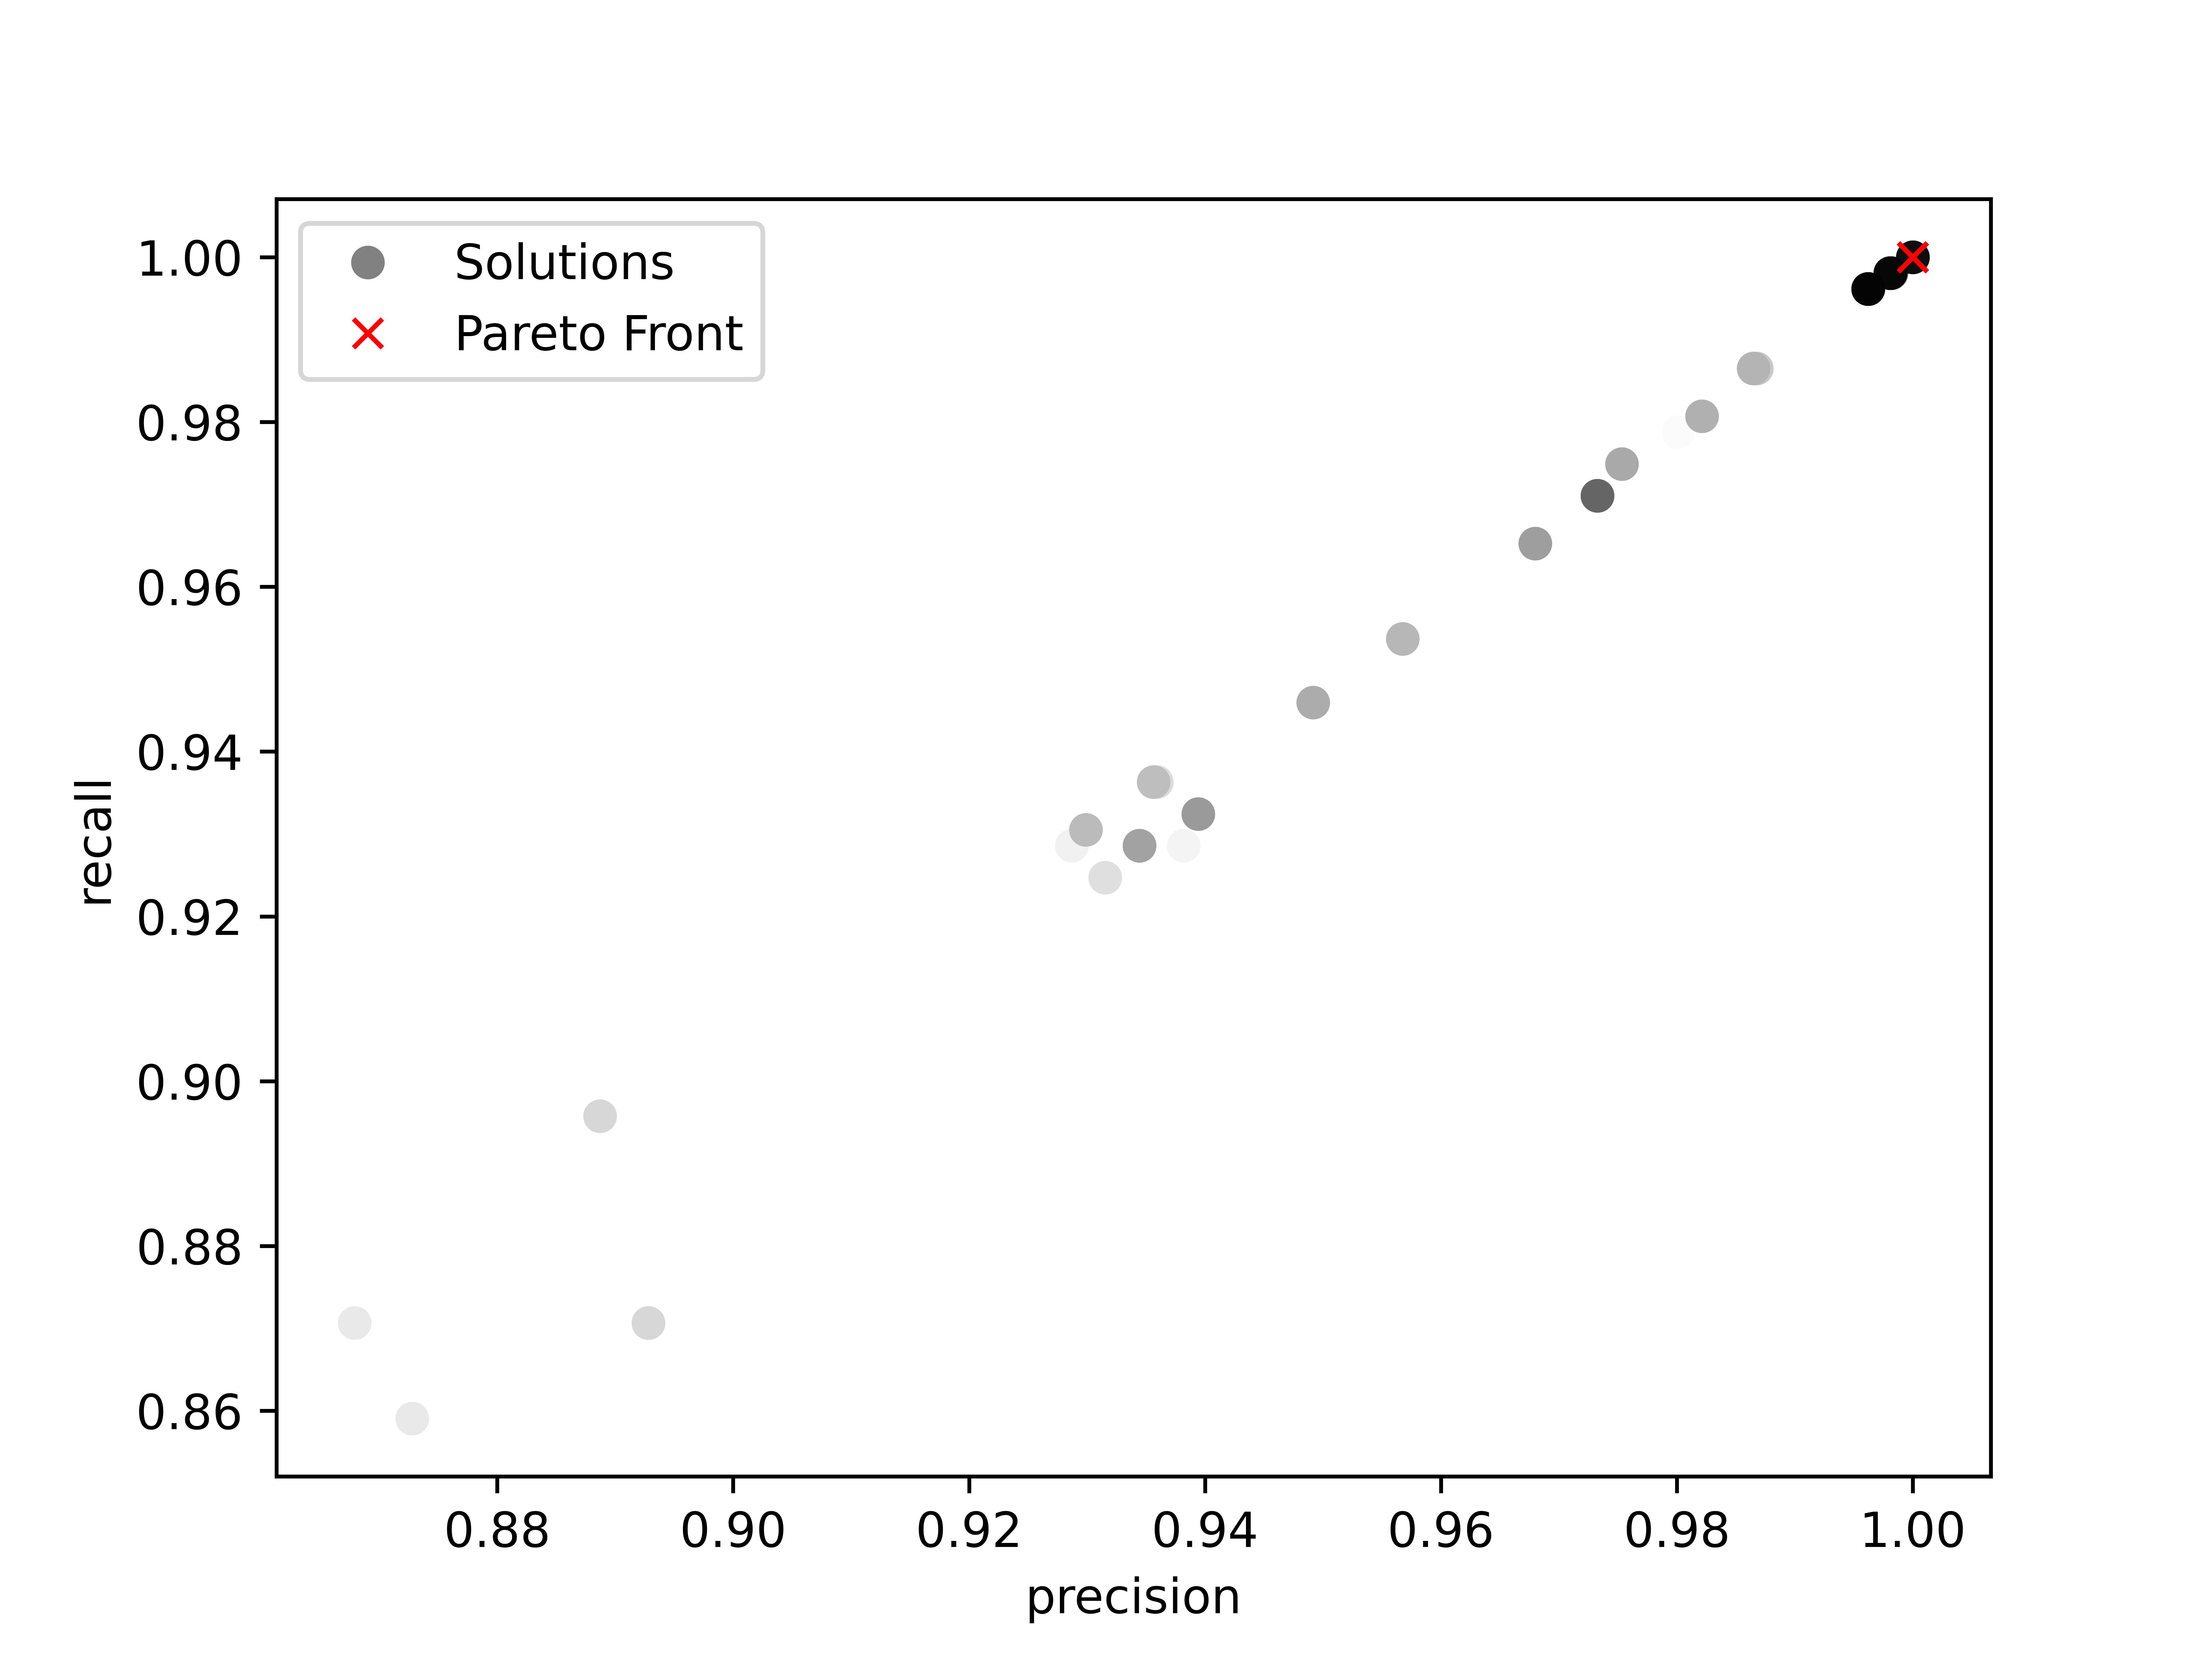
\includegraphics[width=\linewidth]{Pictures/cars_precision_vs_recall.jpg}
    \caption{Cars: Precisi\'on contra recobrad}
    \label{impl:fig:cars:precision_vs_recall}
\end{figure}

\subsection{HAHA}

Se utilzo una poblacion total de 40 individuos, 8 horas de tiempo m\'aximo y 10 segundos por  evaluaci\'on. Las implementaciones de F-Score, Precision y Recall son las implementadas en Scikit con un promedio binario (el estandar) ya que es un problema de clasificaci\'on binario.

\subsubsection{F-Score contra Tiempo de Entrenamiento}

En \ref{impl:fig:haha:fscore_vs_time} se observa un frente con una aparente forma similar al de \ref{impl:fig:cars:fscore_vs_time}. Los pipelines de AutoGOAL en esta ocasi\'on est\'an conformados por dos algoritmos principales. Los que contienen poca precisi\'on pero son general m\'as rapidos est\'an conformados por HasingVectorizer y NearestCentroid y  lo que varia entre ellas son los hiperparametros. Los que tienen mayor precision a costo de un poco de tiempo est\'an compuestos por count vectorizer  y regresores log\'isticos.

Adem\'as en la esquina superior izquierda se ve como AutoGOAL busca un punto que tiene f-score 0, cosa que es completamnete innecesaria, pero el algorimto es agn\'ostico a esto. Ser\'ia recomendable añadir posibles restricciones a las b\'usquedas multiobjetivos para que el algoritmo no pierda poder de computo en buscar soluciones in\'utiles.

Por \'ultimo note que existen algorimtos usan el tiempo m\'aximo de 10 segundos ya que ese es el tiempo m\'aximo de evaluaci\'on dado. Ser\'ia intersante ver que sucede cuando se remueve esta limitaci\'on.

\begin{figure}[ht]
    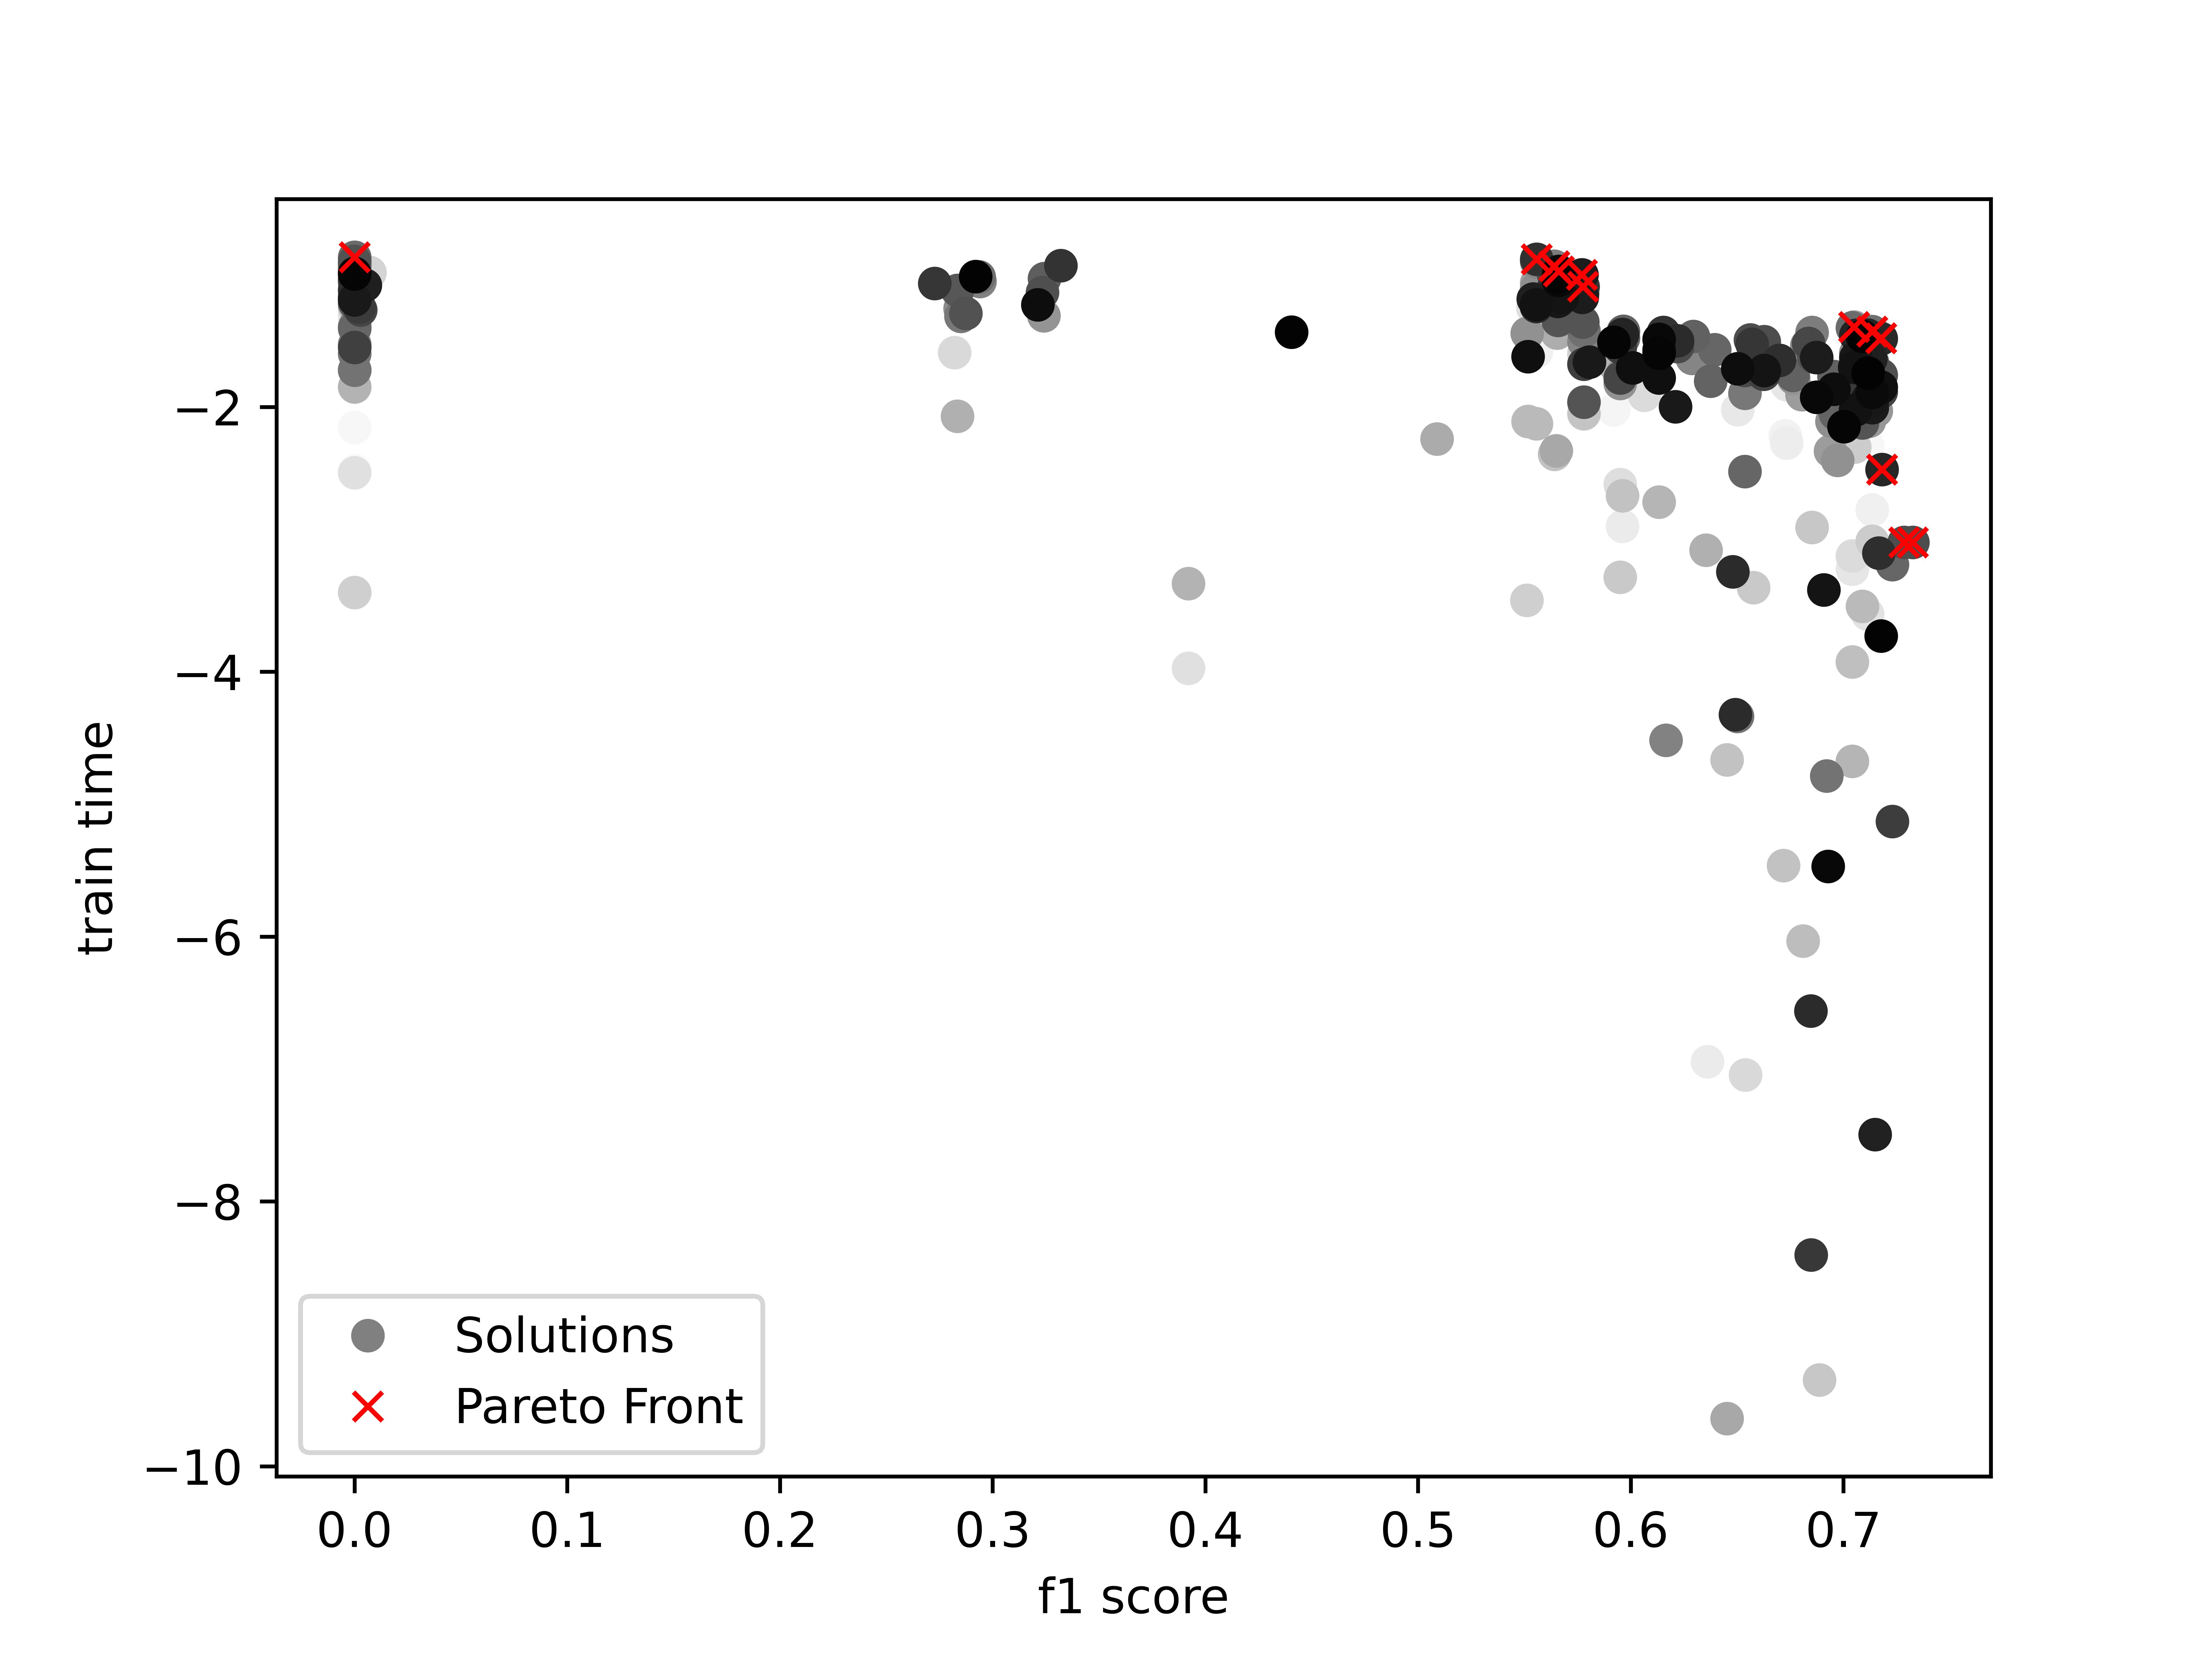
\includegraphics[width=\linewidth]{Pictures/haha_fscore_vs_time.jpg}
    \caption{HAHA: F-score contra tiempo de entrenamiento}
    \label{impl:fig:haha:fscore_vs_time}
\end{figure}
\subsubsection{Precisi\'on contra Recobrado}

Contrario a lo que muestra la evaluaci\'on de Cars con respecto a precision y recobrado, no es posible encontrar un flujo que maximice a ambas y se empiezan buscar modelos que ofrezcan trade offs. Se pueden encontrar con buen recobrado y mala precision, dando y dando, o mal recobrado y muy buena precisi\'on. Este tambien tiene la forma de un frente convexo .

\begin{figure}[ht]
    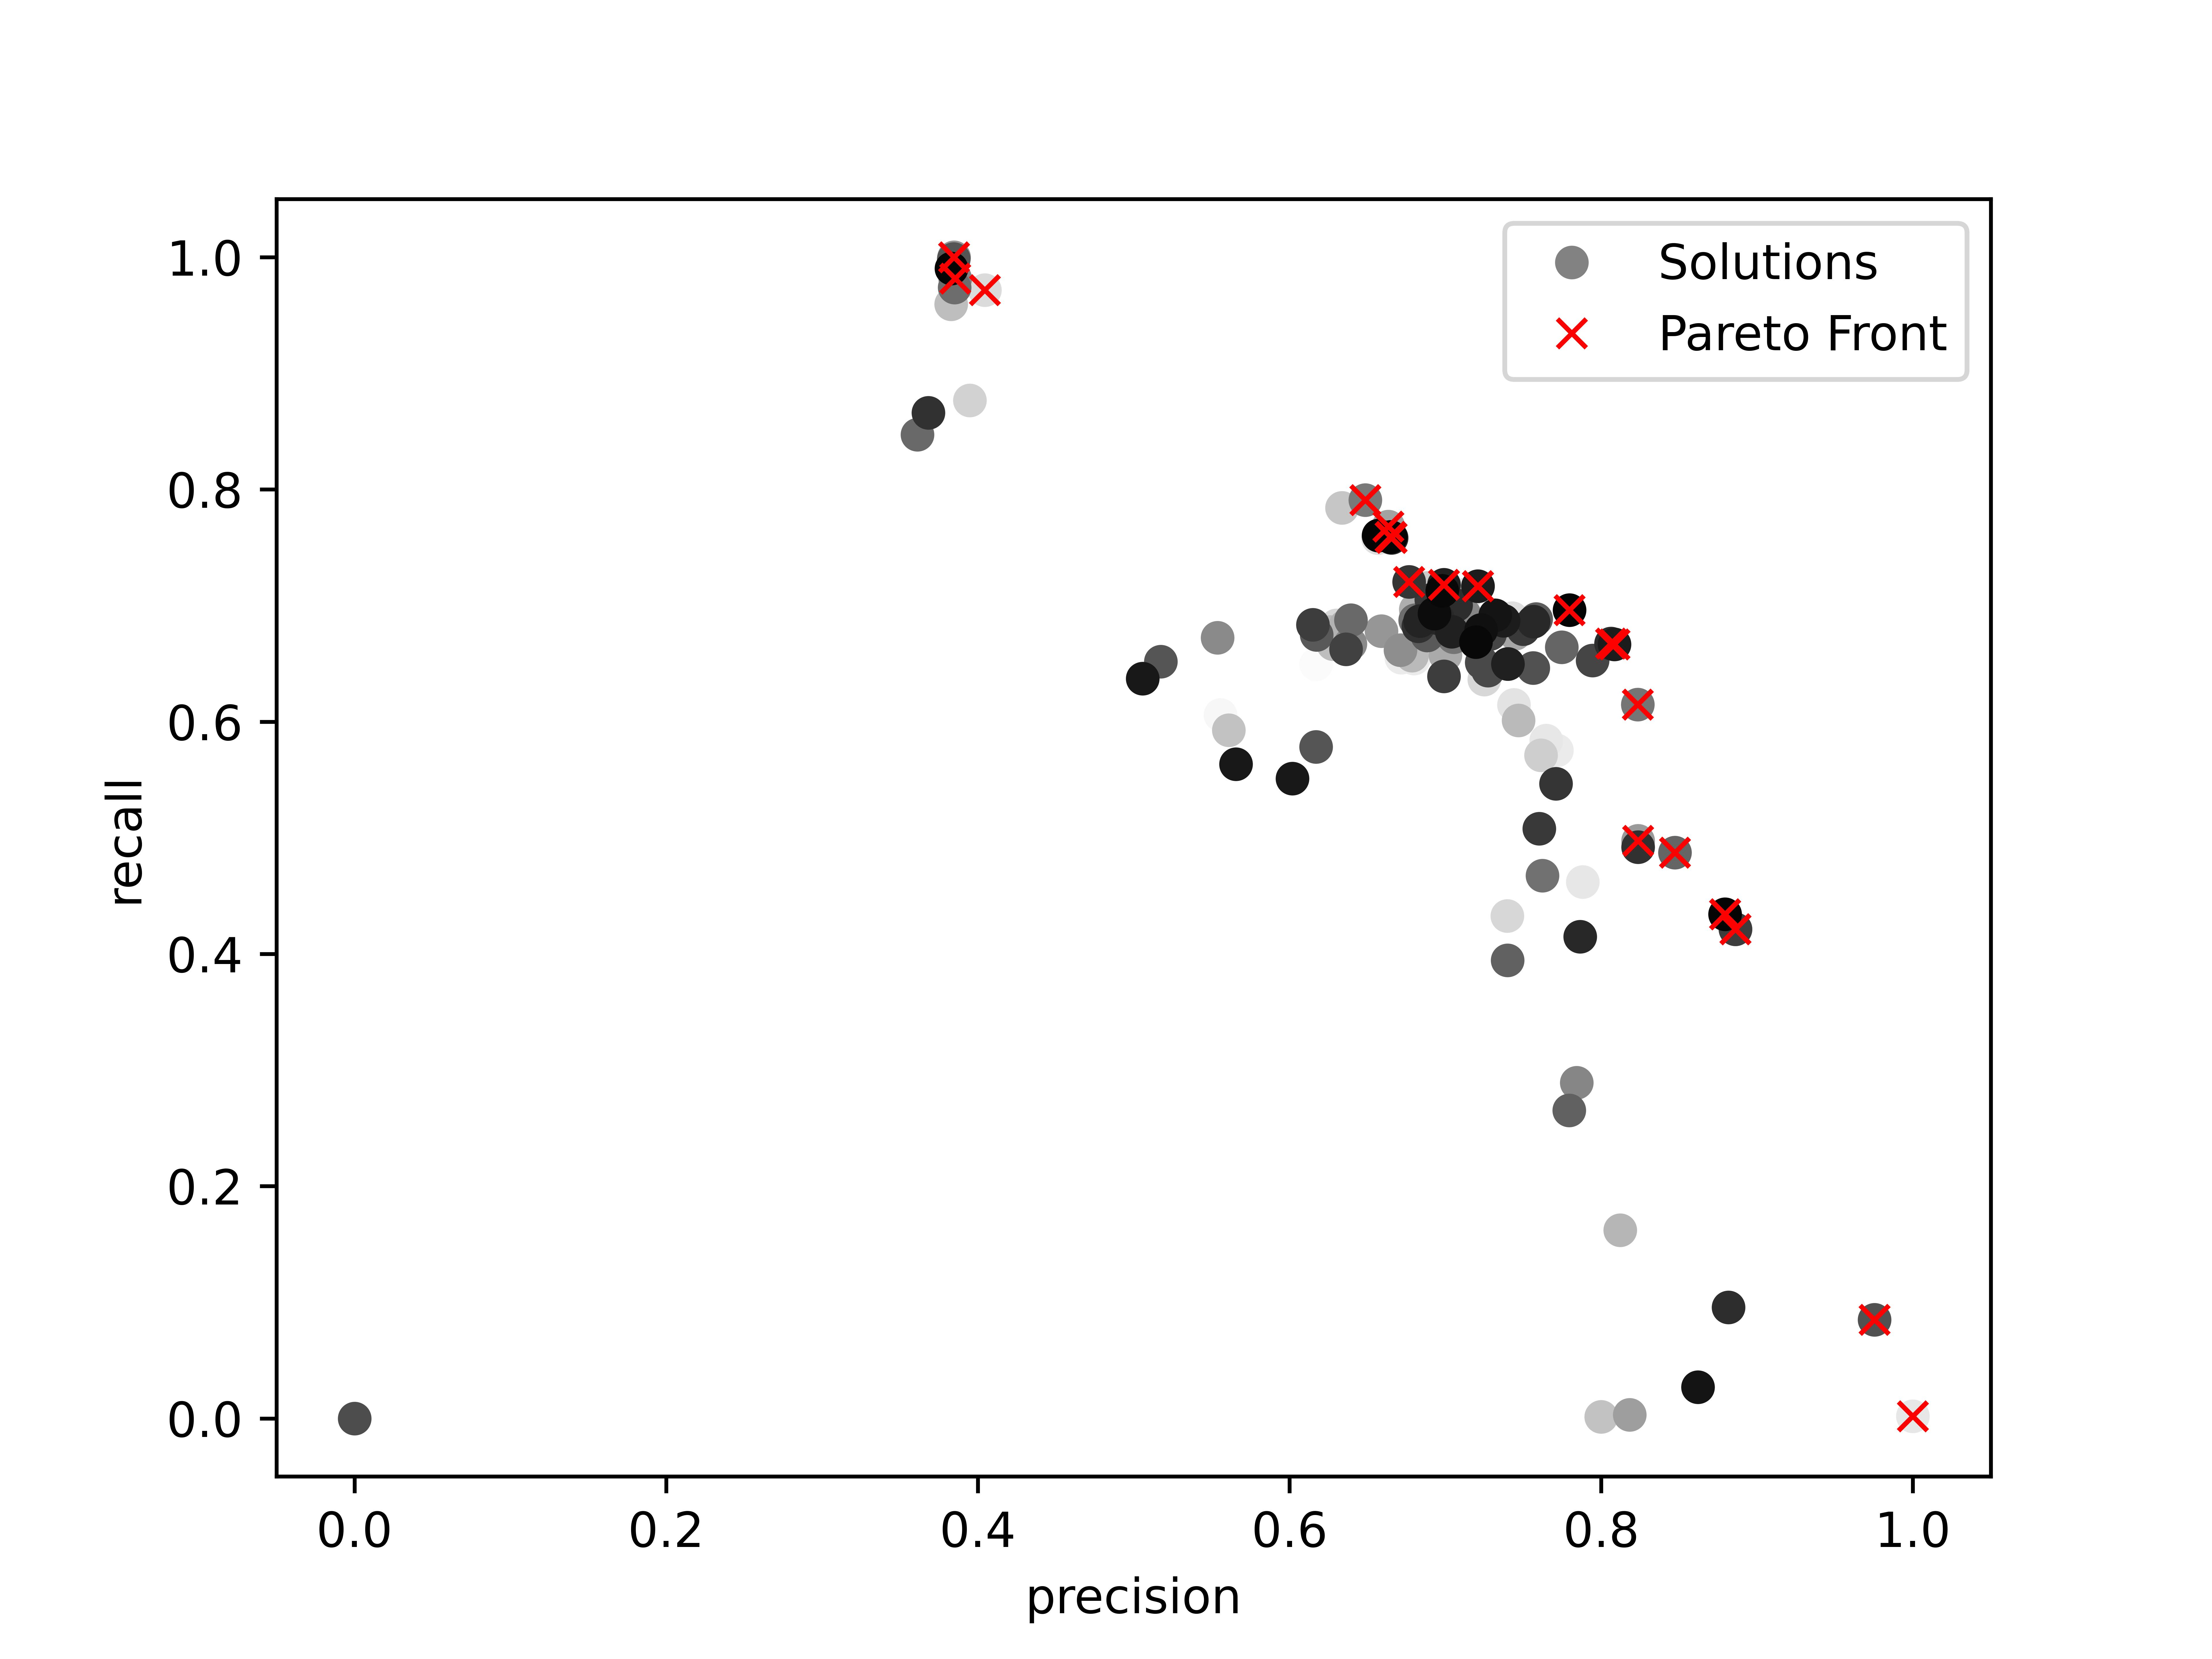
\includegraphics[width=\linewidth]{Pictures/haha_precision_vs_recall.jpg}
    \caption{HAHA: Precisi\'on contra recobrado}
    \label{impl:fig:HAHA:precision_vs_recall}
\end{figure}

\subsection{MEDDOCAN}

Se utilzo una poblacion total de 5o individuos, 10 horas de tiempo m\'aximo y 10 mintuos por  evaluaci\'on. Las implementaciones de F-Score, Precision y Recall son las mismas versiones que vienen acompa\~nadas con el m\'odulo de Python que trae consigo el corpus de datos.

Aqu\'i el tiempo m\'aximo es mucho mayor pues es un corpues mucho m\'as grande que los anteriores que para encontrar al menos un pipeline v\'alido require alrededor de 7 u 8 minutos. Lo suficiente para lograr 3 o 4 generaciones de un total de 100.


\subsubsection{F-Score contra Tiempo de Entrenamiento}


\subsubsection{Precisi\'on contra Recobrado}

% Y despues de las pruebas

% Aqui lo que se me ocurre es poner casos de comparacion:
% Probar con tiempo de entrenamiento vs sin tiempo de entrenamiento
% Probar con precision y recall vs fscore
% Probar con otra m\'etrica como Interpretabilidad o Robustez

% Probar cuando se usan varias m\'etricas (para este s\'abado)

% Plotear como se acerca al frente de Pareto
